% arara: pdflatex: {options: [-output-directory=build, --shell-escape]}
% arara: makeglossaries: {options: [-dbuild]}
% arara: biber: {options: [--output-directory=build]}
% arara: pdflatex: {options: [-output-directory=build, --shell-escape]}

% options:
% thesis=B bachelor's thesis
% thesis=M master's thesis
% czech thesis in Czech language
% slovak thesis in Slovak language
% english thesis in English language
% hidelinks remove colour boxes around hyperlinks

\documentclass[thesis=B,czech]{FITthesis}[2012/06/26]

\usepackage[utf8]{inputenc} % LaTeX source encoded as UTF-8
\usepackage[
	backend=biber
	,style=iso-numeric
	,sortlocale=cs_CZ
	,autolang=other
	,bibencoding=UTF8
]{biblatex}
\addbibresource{sources.bib}

\usepackage{graphicx} %graphics files inclusion
\graphicspath{{./images/}}
% \usepackage{amsmath} %advanced maths
% \usepackage{amssymb} %additional math symbols

\usepackage{dirtree} %directory tree visualisation

% todo package
\usepackage{todonotes}

% code snippets
\usepackage[outputdir=build]{minted}

\usepackage{pdfpages}
\usepackage{listings}

% % list of acronyms
\usepackage[acronym,nonumberlist,toc,numberedsection=autolabel]{glossaries}
\iflanguage{czech}{\renewcommand*{\acronymname}{Seznam pou{\v z}it{\' y}ch zkratek}}{}
\makeglossaries

\newcommand{\tg}{\mathop{\mathrm{tg}}} %cesky tangens
\newcommand{\cotg}{\mathop{\mathrm{cotg}}} %cesky cotangens

% % % % % % % % % % % % % % % % % % % % % % % % % % % % % %
% ODTUD DAL VSE ZMENTE
% % % % % % % % % % % % % % % % % % % % % % % % % % % % % %

\department{Katedra softwarového inženýrství}
\title{Systém pro tvorbu a správu evolvabilních dokumentů}
\authorGN{Tomáš} %(křestní) jméno (jména) autora
\authorFN{Starý} %příjmení autora
\authorWithDegrees{Tomáš Starý} %jméno autora včetně současných akademických titulů
\author{Tomáš Starý} %jméno autora bez akademických titulů
\supervisor{Ing. Marek Suchánek}
\acknowledgements{Doplňte, máte-li komu a za co děkovat. V~opačném případě úplně odstraňte tento příkaz.}
\abstractCS{Práce se bude zabývat vytvářením dokumentů. Cílem práce je analyzovat tvorbu dokumentů a na základě analýzy vytvořit návrh řešení pro tvorbu
modulárních dokumentů. Na základě tohoto návrhu bude následně vytvořena aplikace.

Jedná se o webovou aplikaci, která má oddělené grafické a datové prostředí.
V rámci aplikace je možné vytvářet moduly vně repozitářů, ze kterých je poté možné generovat celé dokumenty, dokumenty i jednotlivé moduly podporují verzování
a je možné získat i dokument starší verze ve správném znění.

Vše poté otestujeme a provedeme zhodnocení přínosů a porovnání se závěry analýzy, také se podíváme na možnosti jak aplikaci dále rozšiřovat.}
\abstractEN{This thesis is focusing on creating modular documents. One of our goals is to analyse document creation and base on
that proppose application desing for our application.
From this design we will then create web application with separate frontend and backend.
Users will be able to create modules inside repositories, using these modules are users
able to create and generate documents. Both documents and modules support versioning
and thanks to that, we are able to generate even older versions of our documents.
At the end we tests our solution and evaluate it. We also propose new features that could
be implemented in the future.
}
\placeForDeclarationOfAuthenticity{V~Praze}
\declarationOfAuthenticityOption{4} %volba Prohlášení (číslo 1-6)
\keywordsCS{dokumenty, modulární dokumenty, reStructuredText, AsciiDoc, python, ruby, webová aplikace}
\keywordsEN{documents, modular docments, reStructuredText, AsciiDoc, python, ruby}
% \website{http://site.example/thesis} %volitelná URL práce, objeví se v tiráži - úplně odstraňte, nemáte-li URL práce

\renewcommand\listingscaption{Zdrojový kód}
\renewcommand\listoflistingscaption{Seznam zdrojových kódů}

\newglossaryentry{CVUT}
{
	name=ČVUT,
	description={České vysoké učení technické v Praze}
}
\newacronym{FIT}{FIT}{Fakulta informačních technologií}
\newglossaryentry{xml}
{
	name=XML,
	description={Extensible Markup Language, jazyk použivající se například pro serializaci dat, hojné zastoupení má v internetové komunikaci}
}
\newglossaryentry{html}
{
	name=HTML,
	description={HyperText Markup Language je značkovací jazyk používaný pro většinu webových stránek}
}
\newglossaryentry{pdf}
{
	name=PDF,
	description={Portable Document Format, formát pro přenášení dokumentů mezi zařízeními}
}
\newglossaryentry{jwt}
{
	name=JWT,
	description={JSON Web Token jedná se o přístupová data ve formátu JSON dle specifikace v RFC 7519}
}
\newglossaryentry{orm}
{
	name=ORM,
	description={Object Relational Mapper, neboli propojení objektů z prostředí programu do tabulek v databázi}
}
\newglossaryentry{guid}
{
	name=GUID,
	description={Globally Unique Identifier, jedná se o unikátní identifikátor, který by měl být naprosto unikátní, jinak se také označují jako UUID (Universaly Unique Identifiers)}
}
\newglossaryentry{gdpr}
{
	name=GDPR,
	description={General Data Protection Regulation v překladu obecné nařízení o ochraně osobních údajů, jedná se legislativu EU, kterou přijala i Česká
	republika. GDPR částečně přepisuje původní znění zákona o ochraně osobních údajů z roku 2000}
}
\newglossaryentry{sql}
{
	name=SQL,
	description={Structured Query Language, neboli strukturovaný dotazovací jazyk, využívá se v rámci relačních databází k získávání dat}
}
\newglossaryentry{vcs}
{
	name=VCS,
	description={VCS je zkratkou pro version control systém, což v překladu znamená verzovací systém. Tyto systémy se používájí pro sledování změn
	mezi jednotlivými úpravami souborů}
}
\newglossaryentry{rest}
{
	name=REST,
	description={Representational State Transfer, jedná se o architekturu, která slouží k vytvoření, čtení, uprávě nebo smazání dat ze serveru pomocí HTTP volání}
}
\newglossaryentry{http}
{
	name=HTTP,
	description={HyperText Transfer Protocol je internetový protokol používající se pro komunikaci s webovými servery}
}
\newglossaryentry{api}
{
	name=API,
	description={Application Programming Interface - rozhraní pro programování aplikací, určuje volání, které bude použito pro komunikaci s aplikací nebo knihovnou}
}

\begin{document}
\renewcommand{\thelisting}{\arabic{chapter}.\arabic{listing}}

\begin{introduction}
	S dokumenty se každý z nás setkává každý den, dokonce i teď držíte jeden v ruce. S tím, jak se rozvíjela lidská civilizace,
se také rozvíjelo psaní dokumentů, od rytí znaků do krunýřů až po moderní psaní na elektronických zařízení a možnost jejich šíření po internetu.
Ovšem metoda psaní se nezměnila, dokument pro nás stále představuje jednotný celek. Představte si ovšem následující případ, máme soubor návodů na náš super
produkt, který má ovšem několik verzí, které se liší i jejich instrukčním manuálem. V našich manuálech se ale nachází odkaz na legislativu, která, jak už to tak
bývá, se mění. Abychom aktualizovali naše návody, musíme změnit všechny soubory, které reprezentují jeden návod. To může být časově náročné a je zde větší riziko
chyby. Cílem této práce je změnit pohled na psaní dokumentů. Jednotlivé dokumenty se skládájí z částí, které se vyskytují v různých dokumentech, ale jsou stejné,
jako v případě našeho příkladu s návody. Jednotlivé části se pak dají aktualizovat a tyto změny se pak projeví ve všech dokumentech, změna tedy proběhne
pouze na jednom místě, což sníží riziko chyby a zároveň ušetříme čas.

Tento problém by nám mohly pomoci vyřešit dnes již existující nástroje, které máme k dispozici. V této práci se na některé podíváme a poté navrhneme řešení, založené
na těchto nástrojích.
\end{introduction}

\chapter{Cíl práce}
Cílem této práce bylo vytvořit aplikaci pro správu a úpravu modulárních dokumentů. Před vytvořením aplikace byla provedena
analýza tvorby dokumentů, ve které jsme si probrali
rozdíly mezi monolitickým a modulárním dokumentem. Na to navázala analýza nástrojů na vytváření dokumentů. Zaměřili jsme se na značkovací jazyky,
které se dnes používájí při vytváření dokumentace
jako například docutil pro jazyk Python či AsciiDoc pro jazyk Ruby.
Po této analýze přijde na řadu návrh aplikace, který zde již lehce nastíníme.

Aplikace bude řešit oprávnění uživatelů, přístup do
jednotlivých repozitářů, což jsou složky s jednotlivými moduly. U jednotlivých modulů musíme myslet na jejich verzování, tedy možnost
vracet se zpět v jednotlivých úpra\-vách. Díky tomuto verzování bude možné generování dokumentů i retrospektivně. Dokumenty, které jsou
složeny z jednotlivých modulů, je možné také verzovat a to pomocí revizí, které si budou pamatovat jaké verze modulů byly použity.

Samotná implementace bude rozdělena na 2 části, backend a frontend. První částí je backend, který nám umožnuje přístup k datům pomocí webového aplikačního
prostředí. Backend má také zajišťovat ověřování uživatelů a\linebreak oprávnění a možnost jejich správy. Frontend nám bude zpřístupňovat \mbox{backend}
ve webovém prohlízeči, jedná se ale o samostatnou aplikaci, která pouze komunikuje a získává data z backendu. Dokončenou implementaci podrobíme
testování, zdali vše funguje v souladu s naším návrhem. Závěrem zhodnotíme výslednou aplikaci, jestli se nám podařilo naplnit všechny cíle, které jsme
si vytyčili v návrhu.

\chapter{Historie psaní dokumentů}
Pokud se chceme zabývat psaním dokumentů, je vhodné se nejdříve podívat do historie, na to kdy a jak se začaly psát první dokumenty, jak se psaní dokumentů
měnilo s tím jak se měnila vyspělost lidské civilizace.

V dnešní době má každý z nás možnost vytvořit dokument a sdílet jej s ostatními na celém světe a to všechno v rámci několika okamžiků. Toto ovšem nebylo
vždy možné. Podívejme se, jak jsme se jako lidstvo dostalo od~vyškrabávání znaků do~krunýřů až po dnešní psaní a sdílení dokumentu online.

\section{Od krunýřů ke knihtisku}

Základem každého dokumentu je písmo, písmo jako takové se prvně objevuje už v 7. tisíciletí před naším letopočtem a to v~Číně,
kde se našly kosterní pozůstatky a blízko nich i krunýře želv, na kterých se našlo první písmo. \cite{EarliestWriting} Toto je nejstarší doposud
nalezený artefakt obsahující písmo.

Písmo se o něco později také objevuje v Mezopotámii. Zde se objevuje klínové písmo, které přišlo jako zjednodušení pro piktogramy, které se používali
pro kontrolu obilí a dobytka. Společně s klínovým písmem se nezávysle na sobě rozvíjí písmo i na území starého Egypta, zde v podobě hieroglyfů. Tyto dvě
písma se pak rozšiřují po celém regionu, díky tomu roste v celém regionu efektivita ekonomiky a objevují se první historické záznamy
\cite{MesopotamiaHistory} a také první sepsané zákony.

V Mezopotámii se pro psaní klínového písma používaly hliněné destičky, kdežto ve starém Egyptě se používal papyrus. Papyrus se vyráběl ze stébel šáchoru
papírodárného a byl rozšířen po celém středomoří. Jeho výroba byla zapomenuta okolo roku 1100.

V Evropě se poté rozšiřuje používání papíru, který se k nám dostal z~Číny díky Arabům. Papír byl oproti pergamenům, které jsou vyráběny z~kůže, levnější
na výrobu, ale byl horší kvality, tudíž pro důležité dokumenty se používal pergamen. Do poloviny 15. století se ovšem stále většina dokumentů psala bez
použití sofistikované techniky, vše bylo stále opisováno ručně. To ovšem změnil Johan Gutenberg, který významně zdokonalil knihtisk, který se pak do
konce století rozšířil po celé Evropě. Knihtisk zde byl již dříve, ale Johan přišel s nápadem odlití jednotlivých písmen z~kovu, tím se zvýšila
jejich životnost a díky tomu se snížila cena celého tisku. Snížení ceny mělo za~následek rozšíření knih mezí více lidí a tím i zvednutí gramotnosti
obyvatelstva. \cite{ucebnice1}

\section{Průmyslová revoluce}

Ještě před příchodem průmyslové revoluce se objevují první pokusy o psací stroj a to již v roce 1714, kdy byl v Anglii patentován stroj
\uv{vyrážející písmenka na papír} \cite{FirstTypewriter}, ovšem s psacími stroji měl pramálo společného. O více než 100 let později se
objevuje první psací stroj, který přinesl rozložení kláves, které známe i z dnešních moderních počítačů. Toto rozložení bylo zavedeno kvůli
problémům se zasekáváním znaků při stisku více znaků po sobě, které se nacházely blízko sebe. Psací stroje zde s námi byly po většinu 20. století
a byly nahrazeny až počítači, ale o těch až později. Krom psacích strojů se s průmyslovou revolucí se také rozšiřují možnosti tisku, například roku 1799
si nechal N. L. Robert patentovat vynález stoje na výrobu papíru v tzv. \uv{nekonečném} pásu. \cite{Papir}

\section{Moderní technologie}

První počítače byly masivních rozměrů a zaměřeny pouze na určité početní operace, pro které byly sestrojené, jako například ENIAC, který byl za 2.
světové války na univerzitě v Pensylvánii, zde jej použivala americká armáda pro balistické výpočty. Tento počítač zabíral 185.81 $ m^2 $ plochy. \cite{historyComp} V roce
1947 přichází William Shockley, John Bardeen a Walter Brattain z Bell Laboratiories s vynálezem tranzistoru, pevného elektrického přepínače, který nepotřeboval
vakuum \cite{liveScience} (elektronky, které se používali do této doby, jej ke svému provozu potřebují). Jak je ale patrné z rozměrů takového stroje, je jasné,
že toto zařízení se rozšíření mezi masu lidí nedostálo, ovšem v 70. letech 20. století přicházejí první osobní počítače. Mezi lety 1974-1977 se na trhu objevují
první opravdové domácí počítače jako například Altair od Micro Instrumentation and Telemetry Systems (MITS). \cite{liveScience}

V roce 1976 Steve Jobs a Stephen Wozniak zakládají společnost Apple, jejich prvním produktem je Apple I, narozdíl od Altair měl tento počítač více paměti a levnější
procesor a monitor. O rok později začinají s produkcí Apple II, který nabízel barevnou obrazovku a možnost záznamu dat na přenosné médium, kazetu, která poté byla
nahrazena za disketu. Apple zárověň\linebreak s~vydáním Apple II vyzýval programátory, aby pro své počítače vytvářeli aplikace, díky tomu například vznikl první tabulkový program
nazývaný\linebreak VisiCalc~i~díky tomuto si Apple našel cestu nejen do domácností, ale i do firemního sektoru. \cite{liveScience}
\uv{První zpracovaní textu na počítači se stáva skutečností, když MicroPro International vydává WordStar.} \cite{liveScience}

\subsection{Software}

V dnešní době ale již existuje nepřeberné množství sofwaru na vytvoření a zpracování textu, uveďme si tedy ty nejznámnější i s~jejich krátkou historií. Začneme tedy
tím nejznámnějším, nejpoužívanějším a v dnešním době již braným jako standard, Word přišel na svět v roce 1983 \cite{word83}. Tato verze byla určena pro systém MS-DOS,
MS Office a s ním spojený Word jak jej známe dnes se ovšem objevil až v roce 1990, konkrétně 19. listopadu toho roku. S~jednotlivými verzemi se zlepšovalo grafické
rozhraní pro uživatele, s verzí 2016 přichází také optimalizace na mobilní zařízení a dotykové obrazovky. V roce 2011 je představen Office 365, online služba, ve
které je možné vytvářet a sdílet dokumenty odkudkoliv. \cite{word}

Neboť balíček Office je licencovaný firmou Microsoft a není možné jej používat bez licence, objevují se i open source řešení, mezi nejznámnější patří OpenOffice/LibreOffice,
jejich příběh začíná v roce 1999, kdy Sun Microsystems kupuje Star Division a mění název jejich produktu na OpenOffice.org, zárověň s tím vydávají kód k veřenjnému užití, open source,
každý si tedy může stáhnout kopii tohoto softwaru a užívat je jí volně. V roce 2009 kupuje Sun Microsystems firma Oracle, neboť měli někteří vývojáři z The Document Foundatiuon obavy,
co se stane s OpenOffice.org, vytvořili si vlastní odnož (fork) OpenOffice.org a začali ji dále rozvíjet pod názvem LibreOffice. Později díky tomuto vzniká i jednotný open source
formát pro sdílení dokumentů, Open Document Format (ODF). Díky vývojářům z Document Liberation Project je možné otevírat i ostatní formáty jako je .doc, .docx nebo importovat
soubory z Pages, což je Word v podání společnosti Apple. \cite{LibreHist}

\section{Shrnutí historie}

Jak je vidět, s postupujícím se technologickým rozvojem lidstva přicházelo i spoustu změn týkajících se tvoření dokumentů. Od dřívější víceméně ruční práce, která byla zahrnuta
ve všech aspektech se lidstvo dopracovalo do moderního pojetí, kdy není potřeba šířit dokumenty jejich opisováním a je\linebreak v~možnosti čím dál větší části lidstva vytvářet dokumenty,
které mohou být sdíleny po celém světe v rámci okamžiků díky internetu. Co se ovšem\linebreak nezměnilo, je přístup tvorby dokumentů, stále tvoříme dokument jako jeden celek, o~tom více
až v další kapitole.

\chapter{Analýza tvorby dokumentů}
Historii psaní dokumentů jsme si popsali v minulé kapitole, nyní je čas popsat princip, kterým dokumenty vznikají. Vznik dokumentů totiž také prochází
vývojem, ale tento vývoj přichází až v poslední době s rozvojem informačních technologí. Tvorba dokumentů by se dala rozdělit na dva různé přístupy.
Jeden má za výsledek jeden soubor, který tvoří daný dokument a druhý pouze složí dokument z určitých částí.

Než si ovšem popíšeme tyto dva přístupy, je nutné se podívat jak vlastně dokument vzniká. Nejdříve je nutné vytvořit návrh neboli se také používá
označení draft. Tento draft je pouze základní obrys toho co by měl výsledný dokument obsahovat. Pokud se na dokumentu podílí vícero autorů, je
tento draft kontrolován každým z nich. Z draftu se potom začne rozvíjet výsledný dokument, který se po dopsání předává ke kontrole korektorům,
kde se kontroluje pravopis a stylistika. Po konečné kontrole díla autorem či autory je dílo předáno distributorovi. Celý tento postup
je znázorněn na grafu \ref{fig:linflow}

\begin{figure}[h]
    \centering
    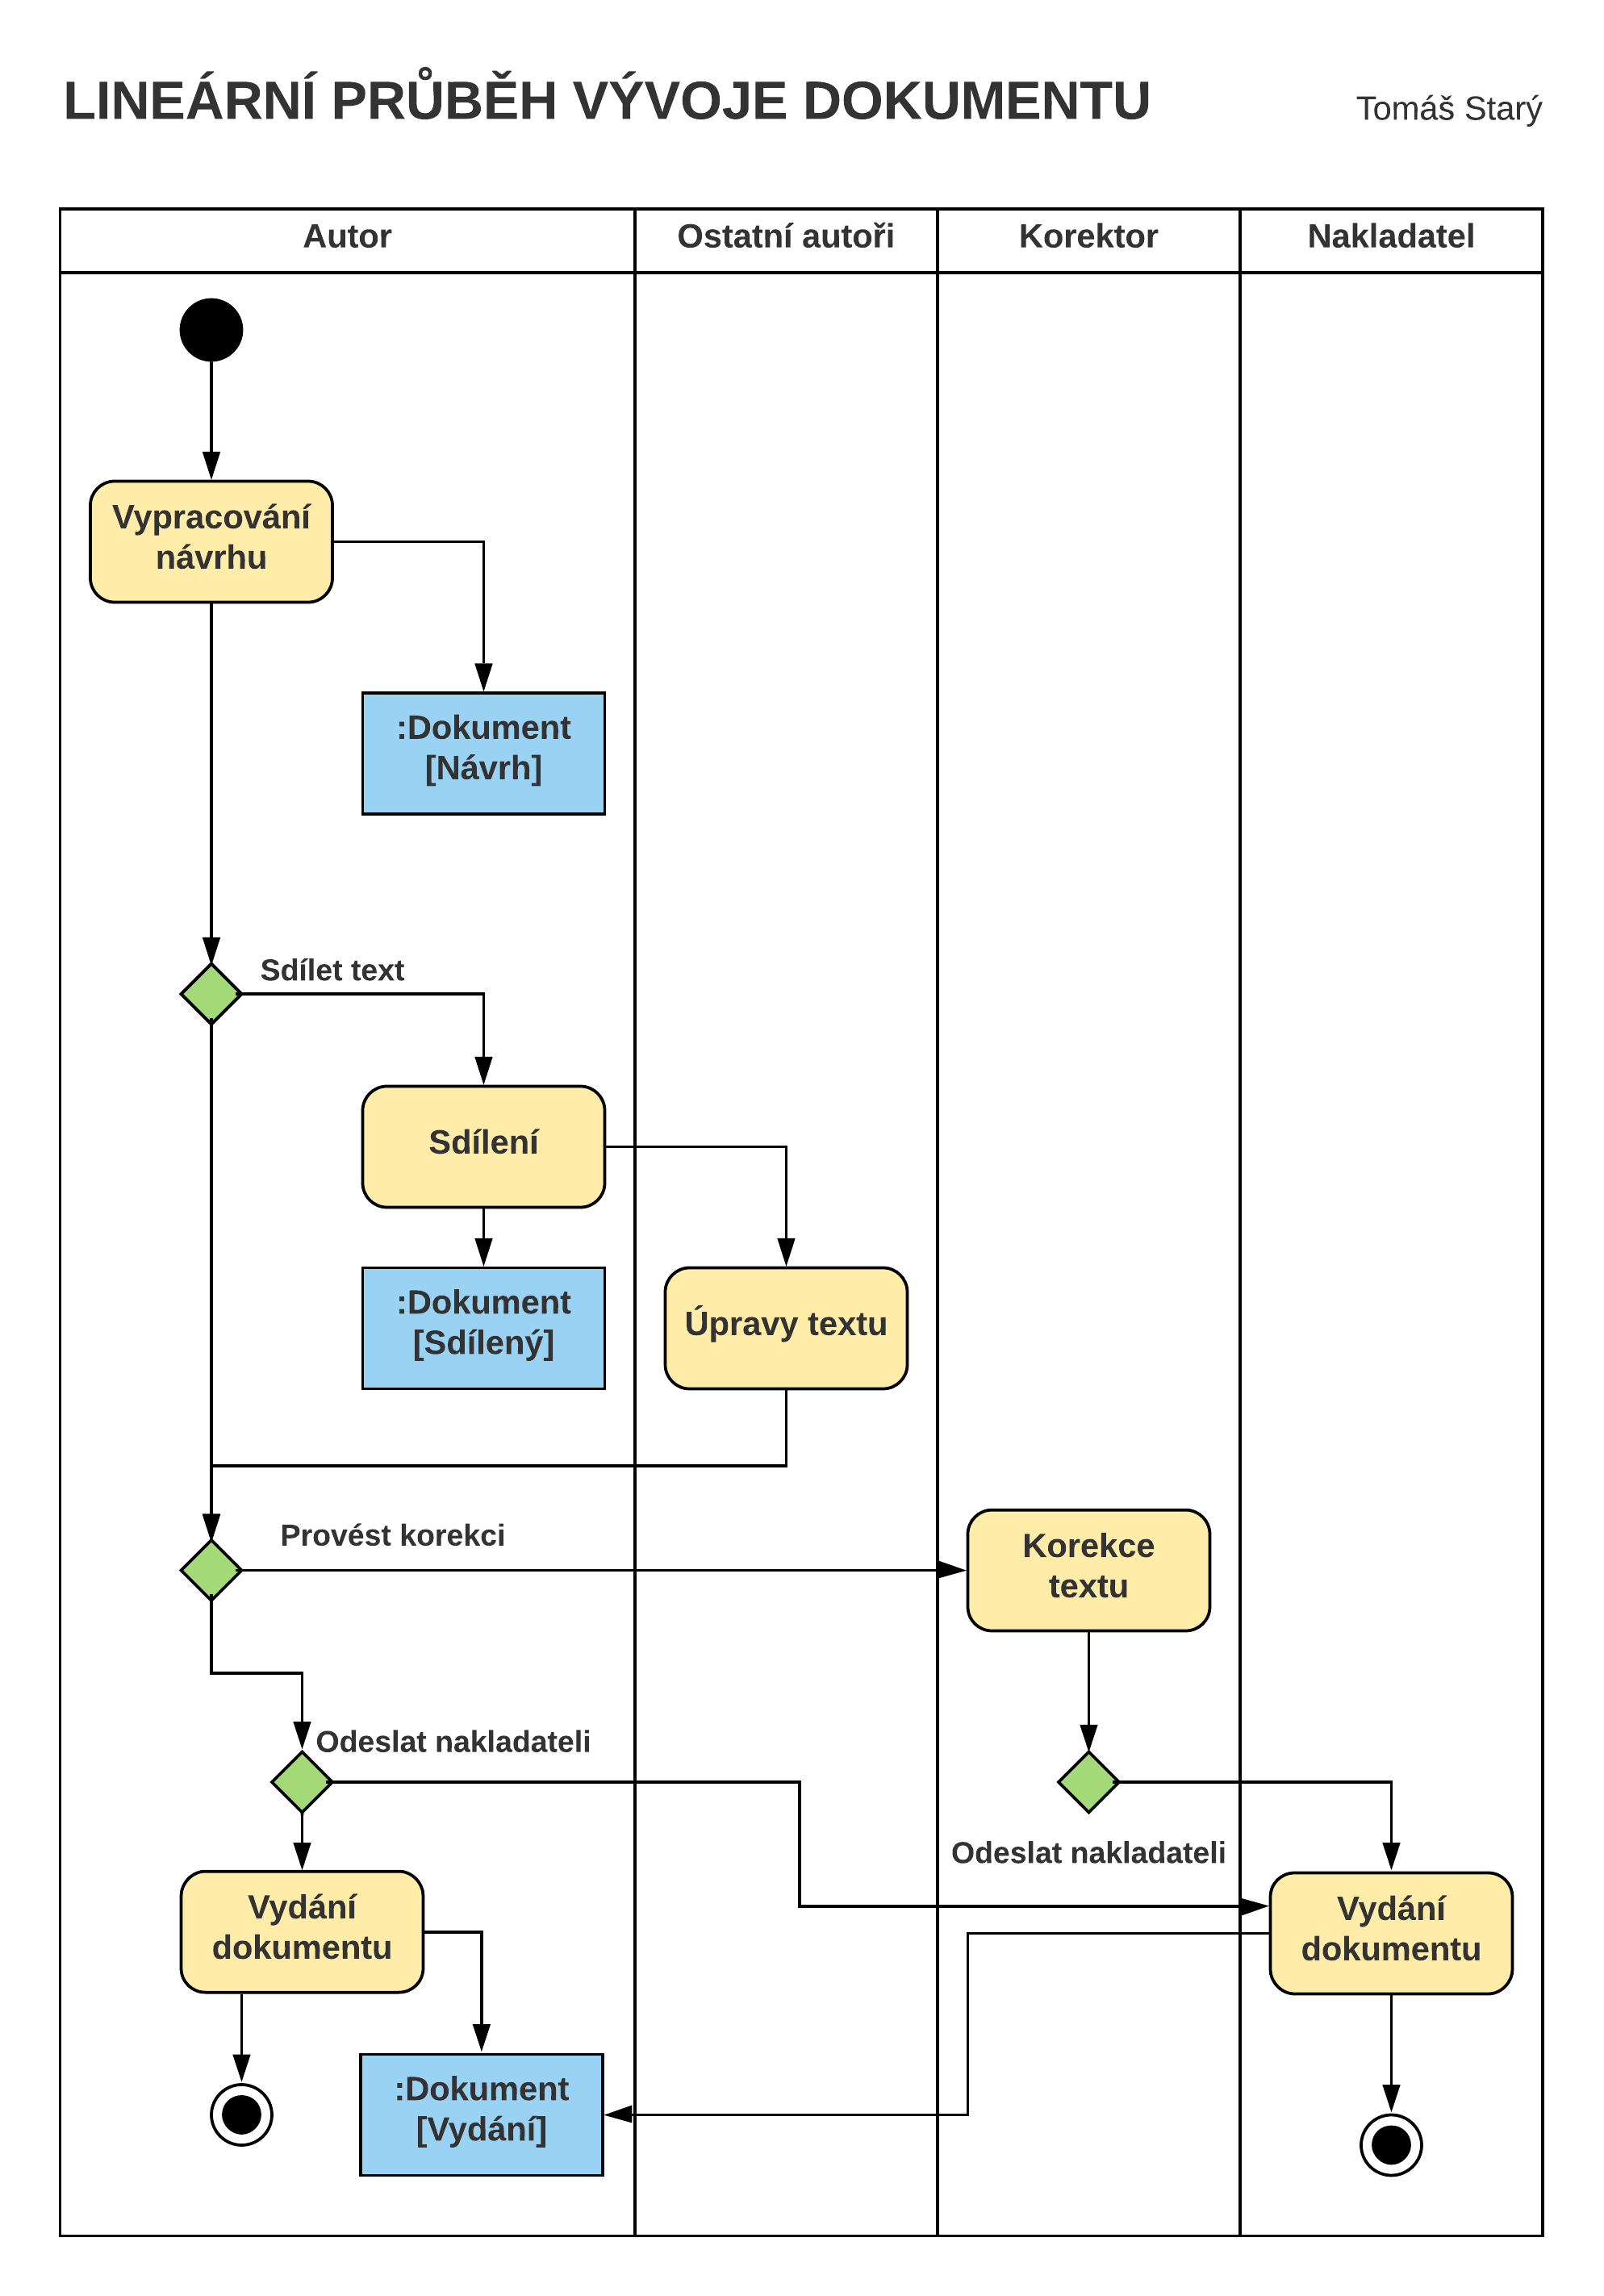
\includegraphics[width=\textwidth]{linearni_prubeh.png}
    \caption{Swimlines diagram}
    \label{fig:linflow}
\end{figure}

\section{Monolitický přístup}

Monolitickým přístupem je myšleno to, že jednotlivé dokumenty jsou jednotné celky, jeden dokument je jeden celek. Pro představu, pokud si vezmeme ku příkladu
Word, o kterém už zaznělo něco v kapitole o historii psaní dokumentů, vytvořením jednoho souboru s příponou .docx, jsme vytvořili jeden monolitický dokument, pokud jej
budeme chtít použít v jiném dokumentu, budeme muset obsah tohoto souboru zkopírovat do nového souboru. Tento nový soubor, který bude obsahovat i náš původní dokument,
pokud se ovšem něco změní v původním dokumentu, druhý dokument bude mít stále původní verzi. Toto poté přináší problémy, které byly již nastíněny v úvodu této práce.

\section{Modulární přístup}




\chapter{Analýza nástrojů pro tvorbu dokumentů}
Nástrojů jak dnes psát dokumenty máme celou řadu, některé jsou volně dostupné a jiné jsou zpoplatněny. Některé nástroje jsme si již představili (Word, LibreOffice), ale
nyní se zaměříme na takzvané značkovací jazyky. Značkovací jazyky nám umožnují psát text, který je poté možné zpracovat počítačem, který změní jeho formátování. Většina
značkovacích jazyků má jasně rozlišitelné značky, nebo jinak také tagy, které upravují formátování při jejich strojovém překladu, díky tomu je původní text stále dobře čitelný.
\cite{markup}

Mezi značkovací jazyky například patří i jazyky používané při psaní webových stránek, jako je HTML či XML, ovšem tyto jazyky budeme spíše využívat pro zobrazování výstupu
jednodušších značkovacích jazyků jako je například Markdown.

\section{Markdown}

Markdown je značkovací jazyk, který převádí text do HTML. Jedná se o jednoduše čitelný a zároveň jednoduchý jazyk na psaní strukturovaného textu. Hlavní myšlenkou Markdown je, že
text v něm psaný by měl být publikovatelný i bez jeho zpracování, inspirací tomuto přístupu jsou čistě textové emaily (emaily se dnes ve většině případů píšou v HTML
z důvodu grafického obsahu). \cite{markdown}

\todo{Místa kde se markdown používá}

Takto vypadá menší ukázka Markdown syntaxe a také výsledek, který je poté generován \ref{fig:markdown}.

\clearpage

\begin{minted}{md}
    # Ukázkový příklad Markdown syntaxe

    Takto vypadá dokument psaný v Markdown,
    jak je vidět, od čistého textu se moc neliší.

    ## Víceúrovňové nadpisy

    *kurzíva*, **tučné**, ~~přeskrtnuní~~

    - příklad
    - jednoduchého
    - seznamu

    - [ ] Checkbox
\end{minted}

\begin{figure}[h]
    \centering
    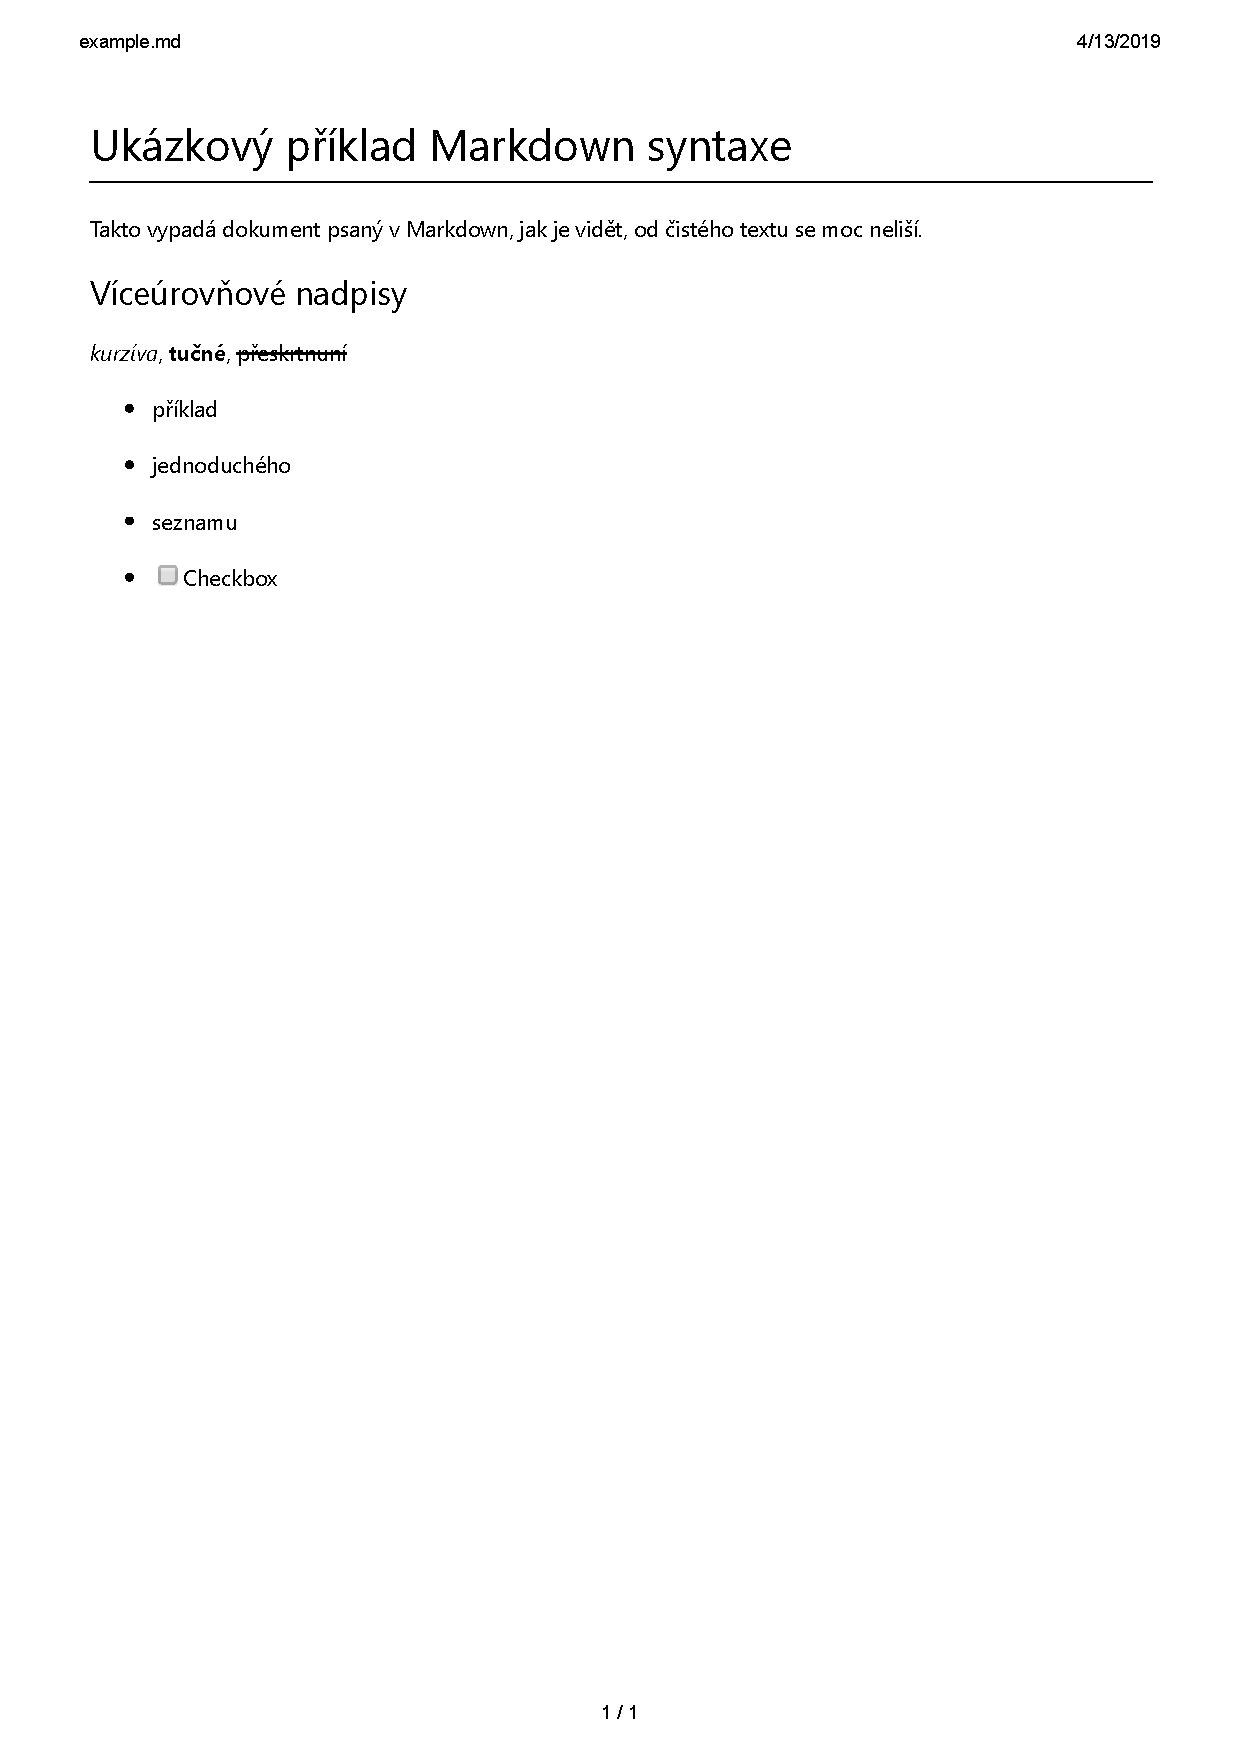
\includegraphics[width=\textwidth]{example.pdf}
    \caption{Výstup Markdown}
    \label{fig:markdown}
\end{figure}

\section{reStructuredText}

Formát reStructuredText pro psaní dokumentů v prostém textu, který je jednoduchý na čtení, kde je hned zřejmé jak bude vygenerovaný text vypadat.
Tento formát je jednoduchý na použití hlavně pro psaní programátorské dokumentace, jednoduchých webů a samostatných dokumentů.
Hlavním cílem reStructuredText je definovat a uplatnit jednoduchý značkovací jazyk pro použítí v Python, kde se používá k dokumentaci jednotlivých částí programu,
a dalších dokumentačních nástrojích, který je jednoduše čitelný a jednoduše použitelný. \cite{reStruDoc}

\inputminted{rst}{example-rst.rst}

\begin{figure}[h]
    \centering
    
\includegraphics[width=\textwidth]{example-rst.pdf}
    \caption{Výstup reStructuredText}
    \label{fig:rstOutput}
\end{figure}

\section{AsciiDoc}

AsciiDoc je další formát pro psaní dokumentu, jedná se stejně jako reStructuredText, o modul pro jazyk Python. Tento modul je možné použít pro psaní nejenom poznámek,
ale je možné jej exportovat i do formátů jako jsou .epub (formát pro elektronické čtečky knih), či PDF. \cite{asciiDoc}

\inputminted{text}{example-ascii.adoc}

\begin{figure}[h]
    \centering
    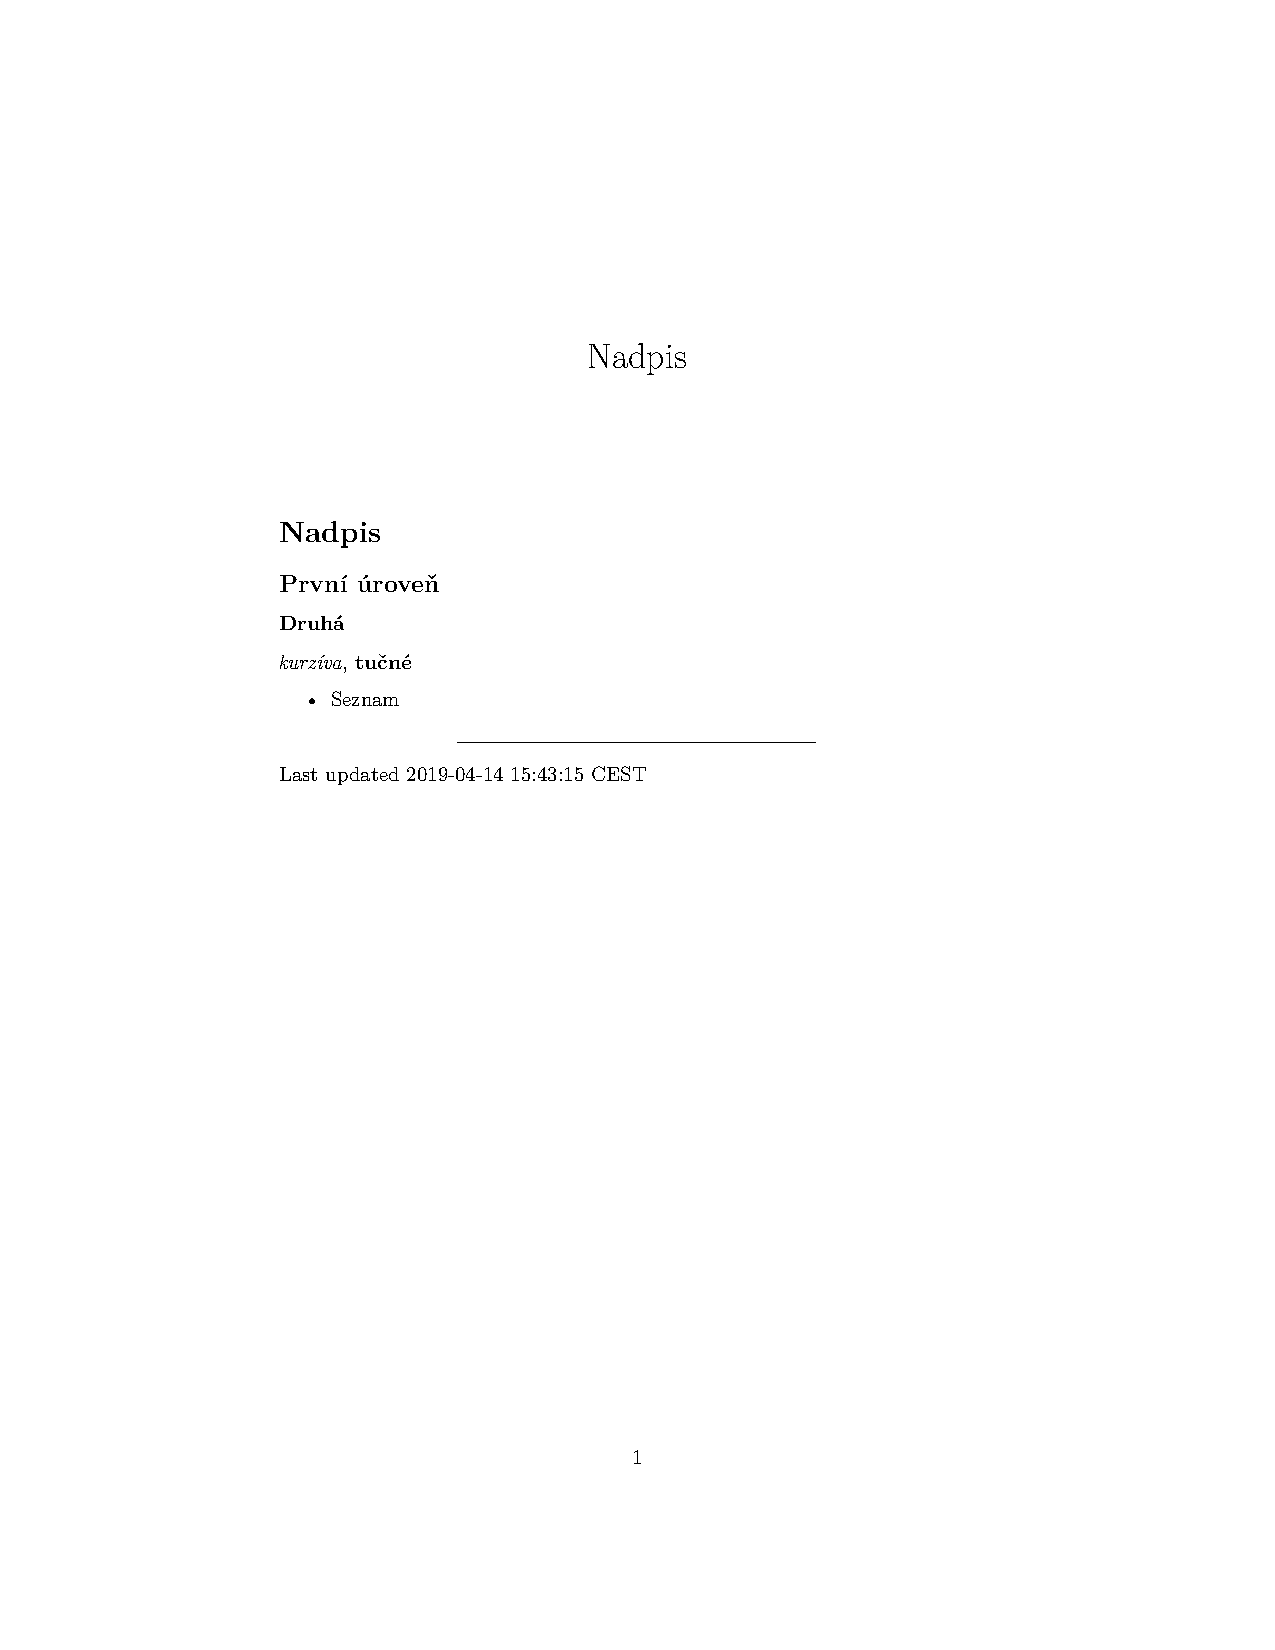
\includegraphics[width=\textwidth]{example-ascii.pdf}
    \caption{Výstup AsciiDoc}
    \label{fig:asciiOutput}
\end{figure}

\chapter{Návrh}
Na základě provedené analýzy máme nyní možnost připravit návrh řešení aplikace, která by zajistila správu modulárních dokumentů, jejich generování/publikaci.
Nesmíme zapomenout na důležité funkcionality. Jedná se hlavně o správu uživatelů, možnost tvořit revize a celkově verzovat jednotlivé části textu.
Dále nesmíme zapomenout na možnost rozšíření aplikace.

\section{Užitelská sekce}

V uživatelské sekci bude hlavní důraz kladen na správu uživatelů, zde také musíme myslet na ochranu jejich osobních udajů a díky GDPR také na
možnost jejich anonymizace. Také je potřeba brát v úvahu rozdělení uživatelů na standardní a administrátorské role, které mají rozdílné oprávnění.
Uživatelem se stává osoba při první interakci s aplikací, v tuto chvíli je osoba brána pouze jako host. Aby se uživatel stal plnohodnotným uživatelem,
je třeba se nejdříve registrovat, tím si uživatel vytvoří vlastní uživatelský účet, který bude mít standardní práva. Pro získání administrátorských
oprávnění je potřeba jiného administrátora, který může běžný účet prohlásit za administrátorský. Ještě bude existovat uživatel se oprávněním
\uv{super admin}, který bude mít práva na všechny operace v rámci systému.

V rámci zjednodušení práce s právy na jednotlivých dokumentech a repozitářích, o kterých se zmíníme později v této kapitole, zavedeme uživatelsky
definované role, které bude poté možné přiřazovat všem uživatelům. Tyto role budou sloužit k hromadným operacím na uživateli, toto ovšem bude
přístupné pouze uživatelům, kteří budou mít roli administrátora.

\subsection{GDPR}

Naše aplikace bude pracovat s osobními údaji a je nutné toto brát na vědomí, proto se nyní podívejme na to, co musí naše aplikace splňovat, aby dodržela všechny
zákony o ochraně osobních údají a směrnice Evropské unie, GDPR. První co je nutné brát na vědomí je účel, za kterým údaje chceme údaje sbírat a uchovávat a jestli je náš
účel oprávněný. V tomto případě o uživateli získáme osobní údaj v podobě emailu, který stačí k identifikaci určité osoby. V našem případě je email identifikátor uživatele
a budeme jej při registraci žádat o souhlas se zpracováním osobních údajů. Dále musíme myslet na možnost smazání či anonymizace údajů uživatele. Toho docílíme ručními
zásahy do databáze, kde využijeme možnosti změnit email na jeho hash. \cite{gdpr}

\subsection{Příklady užití}

Nyní si připomeňme co naše aplikace musí určitě umět z uživatelské sekce, kdokoliv musí mít právo si založit svůj účet a mít možnost se do něho přihlásit.
Po přihlášení musí mít uživatel možnost změnit své vlastní údaje. Pro administrátorské účty musí být zpřístupněna možnost přiřadit role ostatním uživatelům
a zároveň ty role vytvářet, či mazat. Každý uživatel také musí disponovat možností deaktivovat svůj účet. Na obrázku \ref{fig:userFlow} je vidět, jak \mbox{vypadá}
cyklus přihlášení nebo registrace uživatele.

\section{Repozitáře}

Než začneme popisovat samotné generování dokumentů, je potřeba si \mbox{definovat} repozitáře našich modulů. Jednotlivé repozitáře nám budou sloužit jako složky,
které budou obsahovat moduly, ze kterých se pak budou skládat výsledné dokumenty. V rámci repozitářů je potřeba hlavně zajistit správně fungování oprávnění.
Pokud si uživatel založí nový repozitář, má vůči němu všechny práva, ostatní uživatelé se o tomto repozitáři v tomto stavu nemají jak dozvědět, je pro ně
skrytý. Pokud se ovšem zakladatel rozhodne svůj obsah repozitáře sdílet, má možnost sdílet repozitář s jednotlivými uživateli, uživatelskými rolemi a nebo
změnit repozitář na veřejný. Dále má také možnost definovat, jestli je repozitář pro jednotlivé uživatele pouze pro čtení, či použití modulu v dokumenty,
nebo jestli je možnost moduly i upravovat.

V neposlední řadě musíme myslet na verzování našich jednotlivých modulů, zde se nabízejí 2 možnosti jak tomuto přistoupit, buď by bylo možné integrovat
řešení založené na nějaké vcs (version control system), jedná se systém, který zařizuje verzování souborů,
nebo je možné implementovat verzování pomocí databáze. V této práci budeme volit verzování pomocí databáze a to hlavně z časových důvodů, neboť
pro použití vcs by bylo nutné udělat kompletní obal na nějaký již existující verzovací systém. Na digramu \ref{fig:moduleDia} je vidět jak by měly
vypadat vztahy mezi jednotlivými moduly.

\subsection{Přehled všech příkladů užití}

V repozitářích máme 2 hlavní části na které se musíme zaměřit, tou první je nutnost hlídat oprávnění a také je mít možnost spravovat. Tudíž majitel
repozitáře musí mít možnost ovlivňovat, kdo má, či nemá, přístup do jeho repozitáře. Dále musí mít možnost prohlásit svůj repozitář za veřejný a tím
dát možnost všem uživatelům do něj vstoupit. Krom oprávnění je potřeba také zajistit vytváření nových modulů a verzování jejich úprav. U verzování je
potřeba si pamatovat kdo a kdy vytvořil novou verzi. A také možnost vrátit se k určité předchozí verzi.

\section{Dokumenty}

Jelikož už máme definované chování pro jednotlivé repozitáře a jejich moduly, můžeme se vrhnout na návrh dokumentů, které se budou skládat z modulů. Každý
dokument je tedy soubor modulů, který je možné převést do tisknutelné podoby. Na co ale nesmíme zapomenout, že stejně jako moduly bude možné dokumenty také
verzovat, zde to bude provedeno pomocí revizí. Každá revize bude nést informace o tom, kdo danou revizi vytvořil a také ponese všechny informace o verzích
modulu, které jsou na danou revizi použity.

Podobně jako u repozitářů i u dokumentů budeme řešit oprávnění a to stejným způsobem, tudíž každý dokument má svého zakladatele nebo také vlastníka,
vlastník má možnost rozhodovat o tom, kdo bude moci dokument upravovat (vytvářet nové revize, měnit obsah dokumentu), a kdo bude mít možnost si pouze dokument
přečíst. Dále také bude možnost prohlásit dokument za veřejný a bude tedy přístupný všem uživatelům.

\subsection{Příklady užití v dokumentech}

Pro dokumenty bude důležité hlavně možnost jejich generovaní do přenosného formátu, jakým je například \gls{pdf}. Dalším důležitou funkcionalitou bude možnost přiřazování
oprávnění jako je tomu u repozitářů, nesmí chybět ani možnost dokument prohlásit za veřejný a tím jej spřístupnit všem uživatelům. Je také potřeba myslet na možnost
procházet a generovat i starší revize.

\begin{figure}[h]
    \centering
    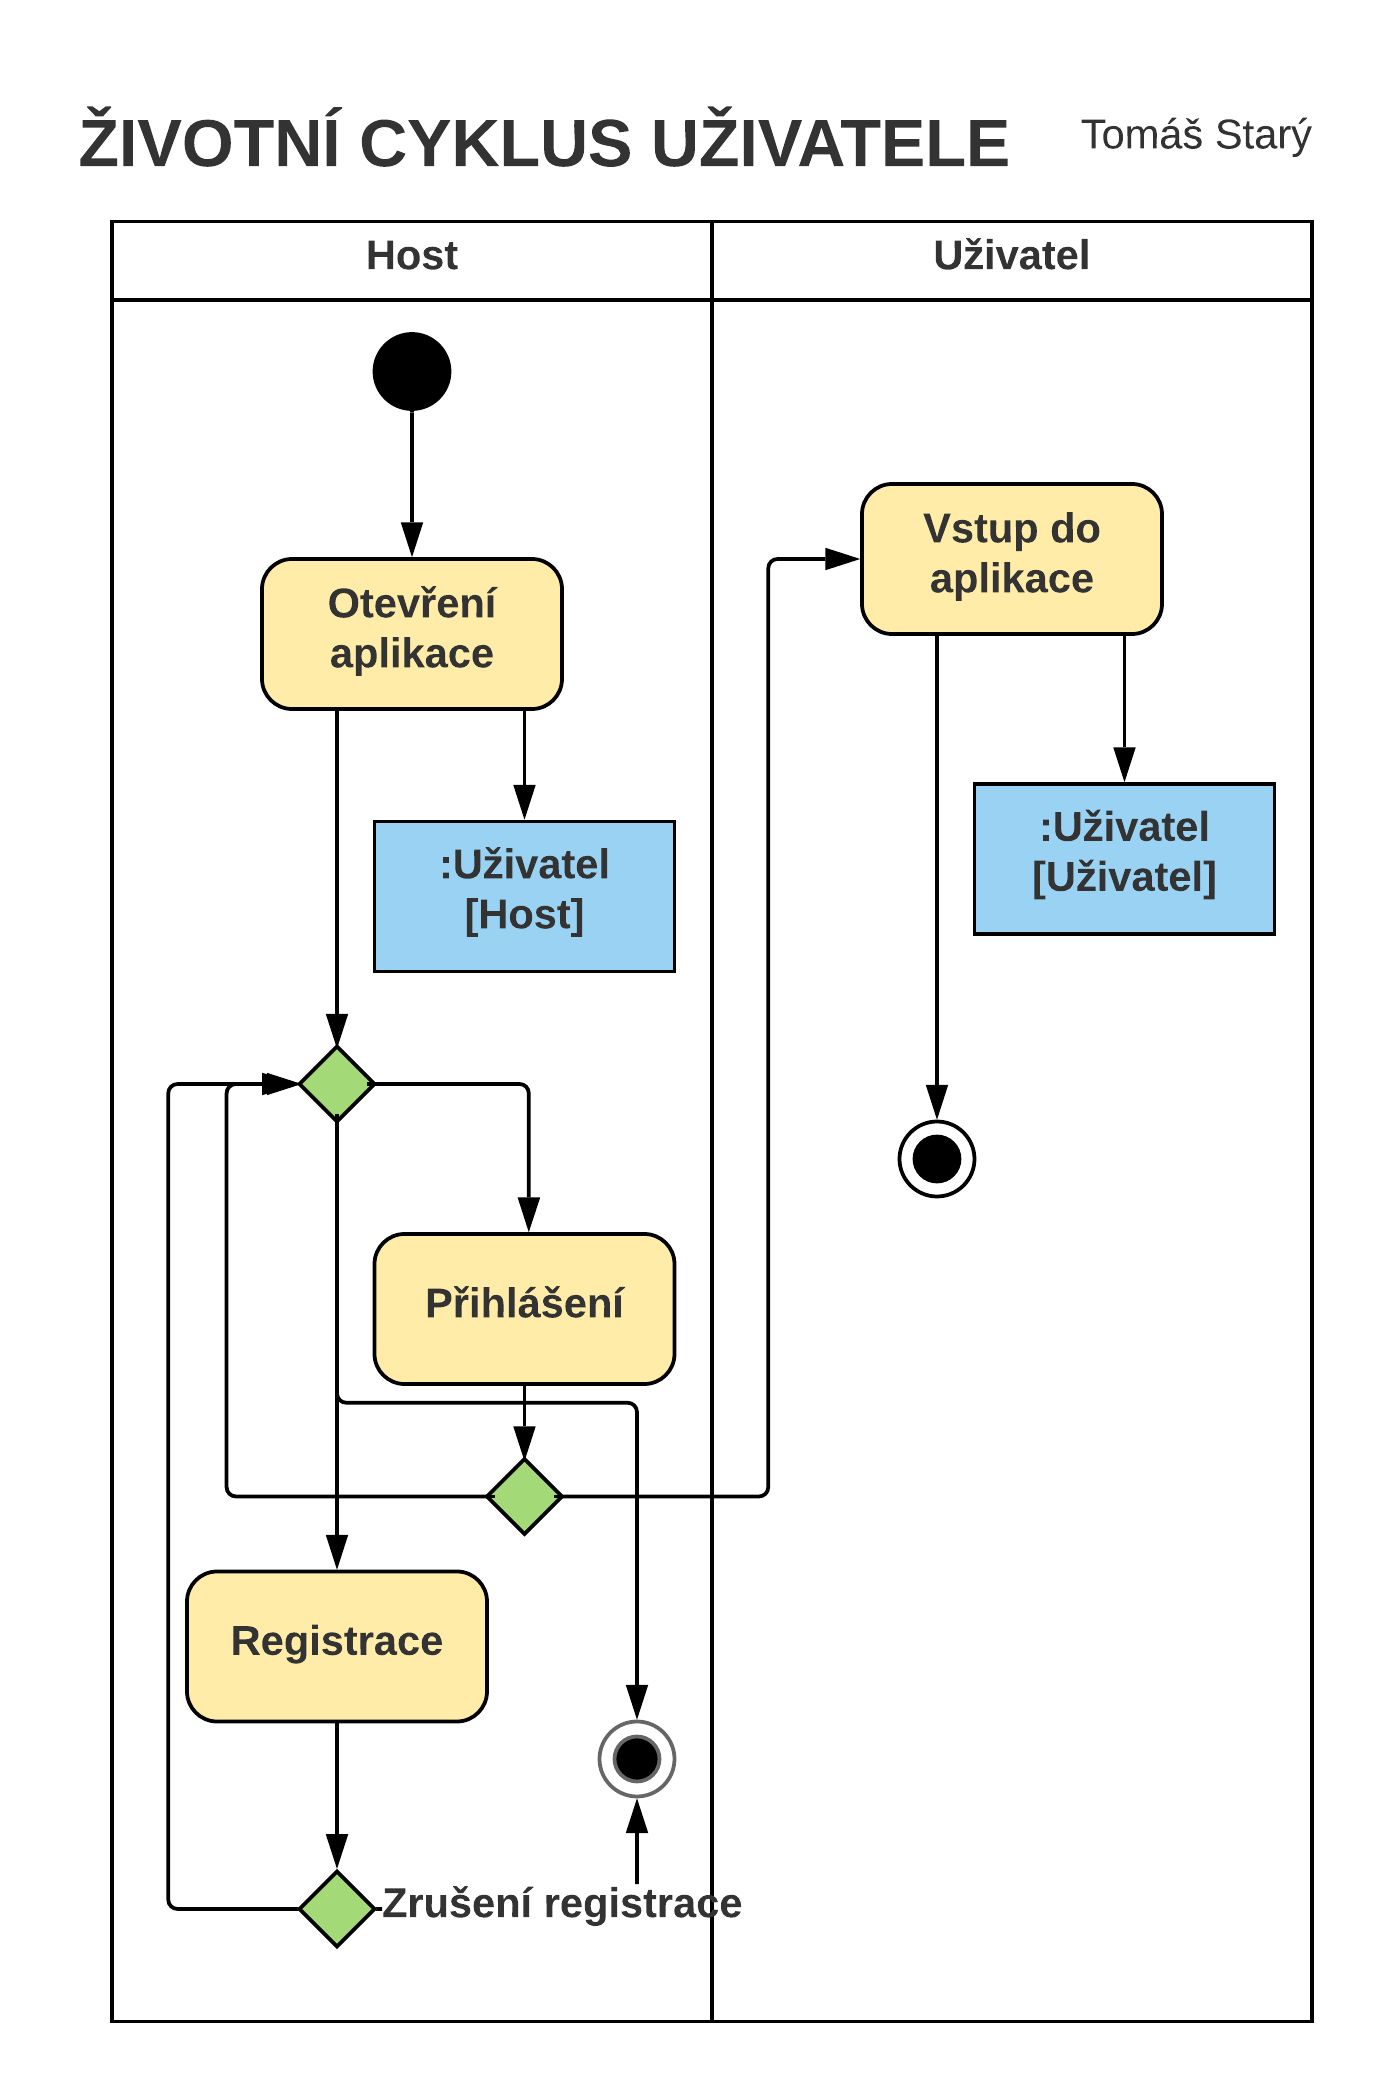
\includegraphics[width=\textwidth]{lifecycle.png}
    \caption{Diagram přihlášení a registrace uživatele}
    \label{fig:userFlow}
\end{figure}

\todo{Odhlášení v diagramu}

\begin{figure}[h]
    \centering
    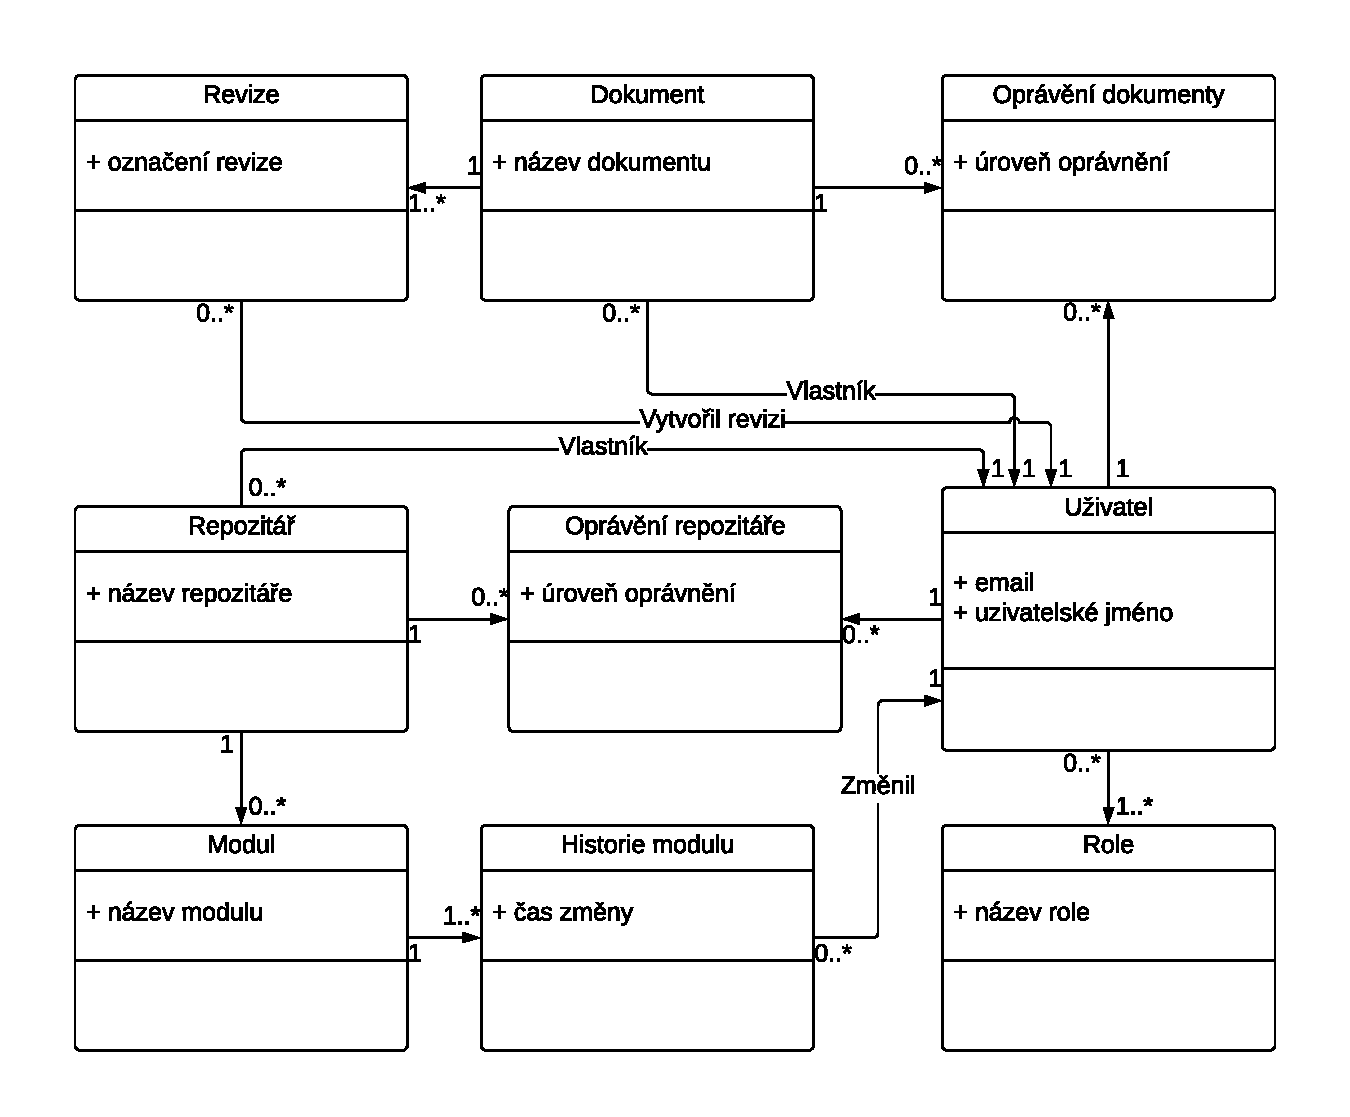
\includegraphics[width=\textwidth]{module_diagram.pdf}
    \caption{Návrh rozložení modelů}
    \label{fig:moduleDia}
\end{figure}

\chapter{Realizace}
Implementaci rozdělíme na 2 části a to na část zabívající se backendem, tedy mozkem naší aplikace, která bude zodpovídat
za ukladání a zpracování dat, bude nám také sloužit jako autentifikační server. A poté na frontend, tedy část, která
je zodpovědné za komunikaci s backendem a také bude zpostředkovávat zobrazení dat z backendu uživateli.

\section{Backend}

Jako základ backendu máme Flask, \uv{což je mikroframework pro Python\linebreak založený na Werkzeug, Jinja 2 a dobrých záměrů.} \cite{flaskDoc}
Tento mikroframework nabízí vytváření stránek ve formátu \gls{html}, toto ovšem nebude třeba, \mbox{neboť} celý backend je složen pouze z \gls{rest} metod,
které slouží k získání či úpravě dat. Konkrétně použijeme HTTP metody GET, POST a DELETE, které provedou určitou akci na základě volané adresy.
Pro další funkcnionality\linebreak využíváme v mnoha případech moduly, které rozšižují základní Flask.

\subsection{Ověřování uživatele}

V rámci ověřovaní uživatelů musíme zajistit zabezpečenou komunikaci mezi backendem a frontendem. Toho docílíme sdílením tokenu, který bude ověřovat
každý dotaz do té části aplikace, kam mají přístup pouze přihlášení uživatelé. Toho docílíme pomocí modulu, který rožšiřujeme Flask,
\textit{Flask-jwt-extended}. Pro správnou funkci tohoto modulu je třeba mít nastavený tajný klíč pro aplikaci, který slouží k šifrování \gls{jwt},
ve kterém se nachází identifikátor uživatele. Dále je potřeba definovat funkce pro načítání uživatele a jeho rolí, toto bude poté použito pro kontrolu
oprávnění uživatele a získávání dat, která jsou vázána na uživatele, zde je ukázka \ref{lst:flaskJWTCode}.

\begin{listing}
    \begin{minted}{python}
        # File: moddoc/service/auth_service.py

        @app.jwt.user_claims_loader
        def add_claims(user):
            """
            Load claims into JWT
            """
            return {'roles': user['roles']}

        @app.jwt.user_identity_loader
        def load_user(user):
            """
            Function for loading user
            """
            return user
    \end{minted}
    \caption{Ukázka kódu pro \textit{Flask-jwt-extended}}
    \label{lst:flaskJWTCode}
\end{listing}

\subsection{Propojení s databází}

Na toto použijeme další rozšíření pro \textit{Flask} a to konkrétně \textit{Flask-SQLAlchemy}, jedná se interpretaci \textit{SQLAlchemy}, což je \gls{orm} nástroj pro Python.
Podporuje většinu \gls{sql} implementací a serverů. V našem případě budeme brát \textit{postgresql} jako nejvhodnější jazyk a databázový server se zaručenou podporou pro \textit{sqlite}. Protože
v aplikaci používáme jako identifikátor všech modelů používáme \gls{guid}, základní implementace \textit{SQLAlchemy} nám ovšem tento datový typ nativně nepodporuje, stejně jako
některé \gls{sql} servery. Proto si vytvoříme vlastní datový typ \gls{guid}, ukázku jak na to nalezeme i v oficiální dokumentaci \textit{SQLAlchemy} \cite{sqlalchemyGuid}. Jak lze
vidět v ukázce kódu \ref{lst:guidImplementation}, při vytváření tohoto typu je provedena kontrola, na s jakou databází bude aplikace pracovat a podle toho se rozhodne jaký datový typ
bude v rámci databáze použit. Toto se provádí protože ne všechny databáze si umí poradit s GUID datovým formátem.

\begin{listing}
    \begin{minted}{python}
        from sqlalchemy.types import TypeDecorator, CHAR
        from sqlalchemy.dialects.postgresql import UUID
        import uuid

        class GUID(TypeDecorator):
            """Platform-independent GUID type.

            Uses PostgreSQL's UUID type, otherwise uses
            CHAR(32), storing as stringified hex values.

            """
            impl = CHAR

            def load_dialect_impl(self, dialect):
                if dialect.name == 'postgresql':
                    return dialect.type_descriptor(UUID())
                else:
                    return dialect.type_descriptor(CHAR(32))

            def process_bind_param(self, value, dialect):
                if value is None:
                    return value
                elif dialect.name == 'postgresql':
                    return str(value)
                else:
                    if not isinstance(value, uuid.UUID):
                        return "%.32x" % uuid.UUID(value).int
                    else:
                        # hexstring
                        return "%.32x" % value.int

            def process_result_value(self, value, dialect):
                if value is None:
                    return value
                else:
                    if not isinstance(value, uuid.UUID):
                        value = uuid.UUID(value)
                    return value
    \end{minted}
    \caption{Implementace GUID datového typu}
    \label{lst:guidImplementation}
\end{listing}

\subsection{Kontrola příchozích dat}

Jako v každém programu je potřeba kontrolovat vstupní data, je i v našem případě nutné kontrolovat data, která přijdou z našeho\linebreak frontendu, nebo například z mobilní aplikace,
která se bude připojovat na náš backend. Pro kontrolu dat použijeme implementaci schémat z dalšího modulu pro Python, \textit{marshmallow}. Tento modul nám umožní definovat
nejen formát dat, ale také definuje formát výstupních dat, která budou načtena přímo z~výstupu dotazu nebo objektu z~\textit{SQLAlchemy}.

\subsection{Struktura backendu}

Přehlednost kódu je jedna z důležitých vlastností aplikace, kterou je snadné udržovat a rozšiřovat. Tomu může i velice pomoct přehledná a intuitivní adresářová struktura.
V rámci backendu máme ještě možnost rozdělit si tuto strukturu podle jednotlivých vrstev, které se v naší aplikaci objevují. Například databázové modely mohou být ve vlastní složce,
nebo všechny \gls{api} metody lze přesunout do jedné složky a rozdělit do souborů, podle toho, k jaké entitě se dané metody vážou.

\begin{listing}[H]
    \dirtree{%
        .1 migrations\DTcomment{složka s migracemi databáze}.
        .1 moddoc.
        .2 api\DTcomment{složka obahující všechny \gls{api} metody}.
        .2 dto\DTcomment{objekty pro přesun informací mezi databází a uživatelem}.
        .2 model\DTcomment{entity}.
        .2 seed\DTcomment{obsahuje základní set dat pro databázi}.
        .2 service\DTcomment{pomocné služby}.
        .2 \_\_init\_\_.py\DTcomment{základní soubor, obsahuje vytvoření instance Flasku}.
        .2 utils.py\DTcomment{utility použiváné v aplikaci}.
    }
\end{listing}


\section{Frontend}

Základním stavebním kamenem frontendu je knihovna React psaná v JavaScriptu. Tato knihovna nám zajištuje základ pro vytváření webového grafického rozhraní. React rozděluje
jednotlivé prvky z rozhraní do komponent, které se poté dají kombinovat, znovu využívat a dá se u nich definovat\linebreak rozšiřující chování. Na psaní v Reactu není potřeba psaní
si vlastních šablon, vše je psáno přímo v JavaScriptovém kódu. \cite{reactJS} Samotný React ještě rozšíříme o~další důležité knihovny.

\subsection{Redux}

Tím asi nejdůležitějším rozšířením Reactu v této práci je knihovna Redux. Redux je, stejně jako React, také knihovna pro JavaScript. Jeho hlavní funkcí je
ukládání si stavů aplikace, tudíž je možné předem nadefinovat všechny stavy, ve kterých se naše aplikace může objevit a není problém se pohybovat na časové
díky této vlastnosti. Je dobré podotknout, že tyto stavy jsou perzistentní. Pro propojení s Reactem existuje knihovna React-Redux přímo od vývojářů Reduxu. \cite{redux}

\subsection{Reactstrap}

Pro frontend je táké důležité, aby všechny ovládácí prvky byly stejné a celá aplikace měla jednotný design. Reactstrap je knihovna rozšiřující React o komponenty,
které jsou již nastylované a to za použití Bootstrap stylů. Tyto komponenty jsou poté použity v celé aplikaci a díky Bootstrapu nemusíme vytvářet vlastní styly,
pokud si vystačíme s tím, co nám nábízí Bootstrap.

\subsection{Struktura aplikace}

Aby se při vytváření aplikace dalo snáze orientovat v již napsaném kódu, investujeme chvilku času do definování a vytvoření adresářové struktury \ref{dir:frontStruct}. Ta nám
pomůže jednoduše určit, kde se nacházejí jednotlivé části aplikace, je třeba dobré rozdělit části týkající se pouze Reduxu do vlastní složky, či je dobré roztřídit
jednotlivé komponenty podle toho, které části aplikace se týkají.

\begin{listing}[H]
    \dirtree{%
        .1 public\DTcomment{složka obsahující HTML s výsledným JavaScriptem}.
        .1 src.
        .2 \_actions\DTcomment{zde se nacházejí všechny akce volané z komponent}.
        .2 \_components\DTcomment{pomocné komponenty}.
        .2 \_constants\DTcomment{konstanty využivané v Reduxu}.
        .2 \_helpers\DTcomment{pomocné funkce a třídy}.
        .2 \_reducers\DTcomment{Redux reducers}.
        .2 \_store\DTcomment{Redux store}.
        .2 App\DTcomment{základní komponenta}.
    }
    \caption{Adresářová struktura frontendové aplikace}
    \label{dir:frontStruct}
\end{listing}

\chapter{Testování a nasazení}
\section{Testování}

Každou aplikaci je třeba otestovat, ani ta naše není výjímkou. Aplikaci otestujeme pomocí akceptačních testů, jedná se o testy,
které jsou provedeny manuálně před samotným nasazením aplikace na produkční prostředí. Testy jsou prováděny podle příkladů užití z návrhu.
V rámci testování sepíšeme jednodtlivé scénáře, které uživatel má otestovat, na základně výsledků těchto testů poté provedeme potřebné
úpravy aplikace.

\section{Nasazení}

Nasazení aplikací se od sebe trochu liší, proto tuto část rozdělím na 2, ve kterých popíšeme nasazení jednotlivých částí.

\subsection{Backend}

Pro nasazení backendu použijeme knihovnu pro jazyk python, \textit{Setuptools} \cite{setupTools}, tato knihovna nám umožní
jednoduše nainstlovat všechny potřebné balíčky, které budeme potřebovat pro běh naší aplikace. Pro nasazení na server
tedy stačí na serveru spustit příkaz \texttt{python setup.py install}, jedinou podmínkou je přitomnost \textit{Setuptools}
na serveru. Před instalací je také dobré nastavit nové připojení na databázi a bezpečnostní klíč. Toto se provede vytvořením
souboru \texttt{config.py} ve složce \texttt{instance}, kterou je potřeba vytvořit v hlavním adresáři aplikace. Aplikaci je
poté dobré spustit pomocí WSGI serveru \cite{flaskDeploy}.


\subsection{Frontend}

Pro frontend využijeme \textit{webpack}, jedná se o modul, který slouží k vytváření balíčků z našeho zdrojového kódu. Výstupem
\textit{webpack} je JavaScriptový, pro nasazení na produkci použijeme funkci

\begin{conclusion}
	Práci jsme uvedli historií vývoje písma a vytváření písmeností, prošli jsme si dopad moderních technologií na psaní a šíření dokumentů a představili jsme si
některé programy, které se nyní používají. V následůjicí kapitole jsme si popsali rozdíl mezi monolitickým a modulárním přístupem k psaní dokumentů a také si
načrtli jak probíhá psaní nového dokuemntu.

Po tomto následovalo popsaní značkovacích jazyků, které se čím dál tím více používají i mimo programátorskou komunitu. Zde jsme se také podívali na
\textit{reStructuredText}, který jsme použili posléze v naší implementaci. Tím se dostáváme k realizaci naší aplikace, které byla rozdělena na 2 části
pro lepší možnosti rozšíření, či propojení s případnou mobilní aplikací. V části o backendu jsme se zaměřili na jednotlivé propojení modulů a důvody jejich
použití.

Celou práci zakončíme otestováním naší implementace. Zhodnotíme přínosy naší aplikace a také naše řešení podrobíme porovnání se závěrem z naší analýzy. Jako poslední
část této práce vyjmenujeme možná vylepšení, které by bylo dobré v dalším vývoji implementovat, ať již za účelem zjednodušení testování, či zvýšení výkonu.
\end{conclusion}
\printbibliography
\appendix

\printglossaries

\chapter{Obsah přiloženého CD}

%upravte podle skutecnosti

\begin{figure}
	\dirtree{%
		.1 readme.txt\DTcomment{stručný popis obsahu CD}.
		.1 exe\DTcomment{adresář se spustitelnou formou implementace}.
		.1 src.
		.2 impl\DTcomment{zdrojové kódy implementace}.
		.2 thesis\DTcomment{zdrojová forma práce ve formátu \LaTeX{}}.
		.1 text\DTcomment{text práce}.
		.2 thesis.pdf\DTcomment{text práce ve formátu PDF}.
		.2 thesis.ps\DTcomment{text práce ve formátu PS}.
	}
\end{figure}

\end{document}
